% ============================================================
% 分片：s02b  对应原文 PDF 第 7--9 页
% 负责章节：2.1.2 Twisting homomorphisms；2.1.3 Gradings；2.1.4 Equivariant cohomology
% 译者：translator-02   审校状态：初稿
% ============================================================

% ==== 原文 PDF 第 7 页 ====

\begin{figure}[tbp]
  \centering
  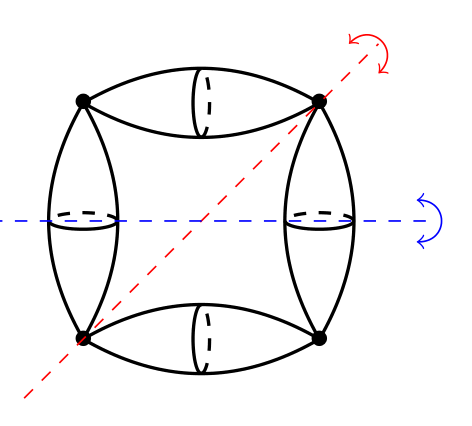
\includegraphics[width=0.92\linewidth]{figures/fig01.png}
  \caption{二维 $\mathcal{N}=(2,2)$ 超对称代数的幂零簇。每个 $\mathbb{P}^1$ 的极点对应秩 1（全纯）超荷，其余各点对应秩 2（拓扑）超荷。红色对称轴对应宇称变换 $(Q_+,\bar Q_+,P_{\bar z})\leftrightarrow(Q_-,\bar Q_-,P_z)$，蓝色对称轴对应电荷共轭 $Q_\pm\leftrightarrow\bar Q_\pm$。（原文第 7 页，Figure 1）}
\end{figure}

\subsubsection{扭变同态}

视所考虑的超荷类型而定，我们可以尝试把扭变后的理论放到与扭变相容的非平凡时空／背景上。对拓扑--全纯混合型超荷，设其有 $n$ 个拓扑方向与 $m$ 个全纯方向，那么至多只能期望把扭变理论放到局部形如 $\mathbb{R}^n\times\mathbb{C}^m$ 的时空上，且其转移函数在 $\mathbb{C}^m$ 上全纯，即 $(x,z,\bar z)\to(y(x,z,\bar z),w(z),\bar w(\bar z))$。这种形式的流形称为具有横截全纯叶理（transverse holomorphic foliation, THF）。例如，可以期望把全纯扭变的理论（$d=2m$）放到一般复流形上，或把拓扑扭变的理论（$d=n$）放到任意流形上。
% [Tutor Note: THF 的转移函数 $(x,z,\bar z)\to(y(x,z,\bar z),w(z),\bar w(\bar z))$ 说明：$x$ 方向只作一般的光滑变换，而 $z$ 方向必须全纯（$w=w(z)$、$\bar w=\bar w(\bar z)$，二者互不混合）。换言之，以 $x$ 参数化的实 $n$ 维叶构成叶理，其叶空间在局部是复流形 $\mathbb{C}^m$——这正是"横截全纯叶理"中"横截"指叶空间方向、"全纯"指横向复结构的含义。复流形本身对应 $n=0$、$m=d/2$ 的特例，故全纯扭变只需复结构、无需更多几何数据。]

在我们的欧几里得框架下，原始物理理论在 $d$ 维平坦空间上具有欧几里得自旋群 $Spin(d)$ 的作用。考虑扭变理论时，超荷 $Q$ 与时空转动不相容：$Q$ 按旋量变换，故 $Q$ 的作用不与时空转动对易。暂设 $Q$ 为拓扑超荷。这一问题的通常解决办法是选取单射群同态 $\iota:Spin(d)\to G_R$，其中 $G_R$ 是物理 QFT 的 $R$ 对称群。若同态 $\iota$ 使得 $Q$ 在经由映射 $\operatorname{id}\times\iota:Spin(d)\to Spin(d)\times G_R$ 给出的 $Spin(d)$ 作用下平凡变换，则可用这一嵌入定义一个与 $Q$ 的作用相容的、修改后的 $Spin(d)$ 作用。我们称之为扭变自旋（twisted spin），并称这样的同态 $\iota:Spin(d)\to G_R$ 为扭变同态（twisting homomorphism）。\footnote{也可以、而且常常有用的是把其他对称性纳入扭变同态。例如，若超对称理论具有内禀对称性 $H$（它必然与 $G_R$ 及 $Spin(d)$ 对易），则可以考虑更一般的同态 $\eta:Spin(d)\to G_R\times H$。为保证修改后的 $Spin(d)$ 作用与扭变相容，需要 $\iota=\pi_1\circ\eta$ 是通常意义的扭变同态。}
% [Tutor Note: 关键在"抵消"：$Q$ 在 $Spin(d)$ 下按旋量表示变换（有非零自旋荷），而在 $G_R$ 下按某个表示（有 $R$ 荷）。沿对角嵌入 $\operatorname{id}\times\iota$ 同时作用，若两种荷之和为零，则 $Q$ 成为该对角作用下的单态（标量），于是"局域转动"可以被 $Q$ 兼容。这正是把自旋群替换为"自旋--$R$ 对称"对角子群的代数实质；$\iota$ 的单射性保证该对角子群同构于原来的 $Spin(d)$，从而不丢失转动信息。]

类似地，若 $Q$ 是一般的拓扑--全纯混合超荷，则只需重新定义与 THF 相容的转动：可以限制到子群 $Spin(n;m)$——我们把它定义为 $Spin(d)$ 中保持分裂 $\mathbb{R}^n\times\mathbb{C}^m$ 的子群——再如上通过扭变同态 $\iota_{\mathrm{mixed}}:Spin(n;m)\to G_R$ 修改这些转动的作用。例如，在最简单的全纯例子 $n=0$、$m=1$ 中没有变化：$Spin(0;1)\cong Spin(2)\cong U(1)$（它是 $\mathbb{C}$ 的转动 $SO(2)\cong U(1)$ 的双重覆盖）。在最简单的混合例子 $n=1$、$m=1$ 中，三维欧几里得自旋群 $Spin(3)\cong SU(2)$ 约化为 $Spin(1;1)\cong U(1)$（即 $\mathbb{R}\times\mathbb{C}$ 中绕 $\mathbb{R}$ 轴转动的 $SO(2)\cong U(1)$ 的双重覆盖）。

% ==== 原文 PDF 第 8 页 ====

再次考虑贯穿全讲的二维 $\mathcal{N}=(2,2)$ 理论这一例子。我们采用的约定是：超荷 $Q_+,\bar Q_+$（相应地 $Q_-,\bar Q_-$）在生成元为 $J$ 的 $Spin(2)\cong U(1)$ 下自旋为 $+\frac12$（相应地 $-\frac12$）。对 $A$ 型扭变（相应地 $B$ 型扭变），典型的扭变同态选取用到矢量 $R$ 对称性 $U(1)_V$（相应地轴 $R$ 对称性 $U(1)_A$），并取扭变自旋生成元 $J_A=J+\frac12 R_V$（相应地 $J_B=J+\frac12 R_A$），使得 $[J_A,Q_A]=0=[J_B,Q_B]$。

在继续之前，我们指出一个小的告诫：这一构造要求底层的超对称 QFT 具有 $R$ 对称群 $G_R$ 的无反常作用，至少对扭变同态中用到的子群无反常。例如，该对称性甚至可能并未在经典层面实现：二维 $\mathcal{N}=(2,2)$ Landau--Ginzburg 模型只有在超势的矢量 $R$ 荷为 2 时才实现矢量 $R$ 对称性。因此，不能在弯曲世界面上考虑它们的 $A$ 型扭变。另一种情形是，经典实现的 $R$ 对称性也可能受量子反常之害：具有一般凯勒靶空间的二维 $\mathcal{N}=(2,2)$ $\sigma$ 模型的经典轴 $R$ 对称性带反常，除非其第一陈类 $c_1$ 为零，即除非它是 Calabi--Yau 的。因此，一般凯勒 $\sigma$ 模型的 $B$ 型扭变与一般世界面不相容。这一现象往往经由镜像对称与前述 Landau--Ginzburg 例子相联系。
% [Tutor Note: 为何超势的矢量 $R$ 荷必须为 2？超势项 $\int d^2\theta\,W$ 中的测度 $d^2\theta$ 带矢量 $R$ 荷 $-2$（两个 $\theta$ 的荷之和），故该项不变要求 $W$ 的矢量 $R$ 荷为 $+2$。若 $W$ 的荷不为 2，则只有 $R$ 对称性的某个子群（至多整体重标度）在经典层面实现，$A$ 型扭变所需的 $U(1)_V$ 便不存在，这正是不能在弯曲世界面上作 $A$ 型扭变的根本原因。]

然而，只要感兴趣的是在平坦空间上研究扭变理论，扭变态射（twisting morphism）的选取就是可选的。\footnote{事实上，全纯扭变的理论可以定义在 Calabi--Yau 流形上；只要扭变态射选取适当，这可以推广到凯勒流形。} 要把理论放到更一般的时空上，就需要扭变同态来保证 $Q$ 的作用与坐标变换相容。更精确地说，扭变超荷作为时空旋量，在具有非平凡自旋结构的时空上会非平凡地变换。为补偿这一点，我们引入背景 $R$ 对称丛，其转移函数恰好抵消自旋结构的转移函数——至少对扭变超荷 $Q$ 而言如此。扭变同态的选取简洁地编码了应引入何种背景：若 $P_{\mathrm{Spin}}$ 是时空上的自旋丛，则我们取 $Spin(d)\times G_R$ 丛，其转移函数由 $P_{\mathrm{Spin}}$ 的转移函数与扭变同态复合给出：即在两个开覆盖片 $U,V$ 上有 $U\cap V\to Spin(d)\xhookrightarrow{\iota}Spin(d)\times G_R$。
% [存疑: 原文此处用 "twisting morphism"，与前文定义的 "twisting homomorphism" 用词不一致，所指应为同一对象；译文保留"扭变态射"以对应原文用词。]
% [Tutor Note: 这里的丛构造不是把结构群"约化"，而是用 $\iota$ 作纤维积：$P_{\mathrm{Spin}}$ 与 $R$ 对称丛沿 $Spin(d)\xhookrightarrow{\iota}Spin(d)\times G_R$ 配对，得到结构群为 $\operatorname{im}(\operatorname{id}\times\iota)$ 的新丛。其转移函数为 $g_{UV}\mapsto(g_{UV},\iota(g_{UV}))$，故 $Q$ 的自旋部分与 $R$ 部分的变换恰好互逆，$Q$ 在该丛上成为良定义的整体对象。核对时应确认 $G_R$ 中 $\iota$ 的像是 $Q$ 的 $R$ 荷所生成的子群。]

更一般地，我们可以要求某个背景（如度规、$R$ 对称丛等）保留一定量的超对称。注意平坦空间的超对称代数与一般时空并不相容——一般度规在由坐标矢量场 $\partial_\mu$ 生成的平移下并非不变，更不用说其超对称扩充了。取而代之，这样的流形可能具有由 Killing 矢量场 $K=K^\mu\partial_\mu$ 生成的等距。类似地，我们可以要求给定背景容许若干（推广的）Killing 旋量场，或简称（推广的）Killing 旋量 $\xi$，满足 $\nabla_\mu\xi\propto\Gamma_\mu\xi$，其中 $\nabla_\mu$ 是背景 $Spin(d)\times G_R$ 丛上的完全协变导数。这些推广的 Killing 旋量与 Killing 矢量场一起生成某个刚性超对称代数。上面由扭变同态实现的代数（至少）有单个与扭变超荷 $Q$ 对应的（推广的）Killing 旋量。
% [Tutor Note: 方程 $\nabla_\mu\xi\propto\Gamma_\mu\xi$ 是（推广的）Killing 旋量方程。比例系数为零时退化为平行旋量（平坦空间超对称），非零时由背景的引力场／通量决定；把"是否存在满足该方程的 $\xi$"作为给定背景保留刚性超对称的判据，就是通常所谓"超对称的刚性极限"的几何表述。]

超对称对给定背景施加的约束，往往可以通过把背景场提升为完整的超多重态、再要求背景费米子的超对称变分消失而容易地读出。在非平凡黎曼流形上工作的语境中，我们把理论耦合到（超引力多重态的刚性极限），并从引力微子的变分读出超对称所施加的约束；这一方法最早由 Festuccia 与 Seiberg 在四维 $\mathcal{N}=1$ 情形中描述 [23]，但可以相当普遍地应用。例如，见 [24] 中各种维度的显式例子，以及同一文集的第 3 篇贡献 [25]，或 [26] 中与二维 $\mathcal{N}=(2,2)$ 理论相关的计算。

% ==== 原文 PDF 第 9 页 ====

\subsubsection{分次}

在 BRST 量子化中，超对称 QFT 有两种自然的分次（grading）或度数；换言之，在取上同调之前，用来刻画理论 Hilbert 空间的复形按（至少）两个守恒荷分层：鬼数（ghost number）$\in\mathbb{Z}$ 与费米宇称（fermion parity）$\in\mathbb{Z}/2\mathbb{Z}$。我们采用如下约定：在代数运算中，符号完全由费米宇称决定。用这些数据来说，BRST 微分 $d$ 的双次数（bidegree）为 $(1,-)$，扭变超荷 $Q$ 的双次数为 $(0,-)$。扭变完成后，理论只保留由费米宇称给出的 $\mathbb{Z}/2\mathbb{Z}$ 分次。
% [Tutor Note: 双次数中的第二个分量写作"-"表示"费米宇称奇"，而非零或负一：BRST 微分 $d$ 提高鬼数 1、且为 Grassmann 奇；扭变超荷 $Q$ 不改变鬼数、同样为奇。因此 $(1,-)$ 与 $(0,-)$ 分别对应"鬼数 +1、宇称奇"与"鬼数 0、宇称奇"。若把"-"误读为 0，就会错误地认为 $Q$ 与 $d$ 同次，从而算错扭变上同调的分次。]

当存在扩充超对称时，我们可以做得比这稍好一些。选取映射 $\gamma:U(1)\to G_R$ 进入 $R$ 对称群 $G_R$\footnote{上述告诫再次略有体现：我们还需要底层超对称 QFT 具有由 $\gamma$ 生成的 $U(1)$ 子群的无反常作用。与上面关于扭变同态的讨论不同，缺少这些 $R$ 对称性并不会使理论不自洽，只是对扭变理论的控制更少。}，使得 $Q$ 在该 $U(1)$ 作用下的荷为 $+1$，且由 $\gamma$ 给出的 $U(1)$ 分次（也称为 $R$ 荷）与费米宇称分次模 2 一致，即若相应生成元记为 $R$，则 $(-1)^R=(-1)^F$。这样的选取使扭变理论具有完整的 $\mathbb{Z}$ 分次（只要所有 $R$ 荷都是整数），它由鬼数（由算子 $\operatorname{gh}$ 度量）与 $R$ 荷（由算子 $R$ 度量）之和给出，我们称之为上同调分次（cohomological grading）：$C=\operatorname{gh}+R$。\footnote{也可以考虑包含内禀对称群 $H$ 的上同调分次。注意修改后的时空转动应具有上同调度 0，即扭变自旋生成元应与度量上同调度数的生成元 $C$ 对易。} 此外，由于 BRST 场的鬼数与宇称相关——例如 $c$ 鬼场的 $(\operatorname{gh},R,(-1)^F)$ 荷／度为 $(1,0,-)$——在这种情况下，上同调分次决定了费米宇称。
% [Tutor Note: 条件 $(-1)^R=(-1)^F$ 保证"$R$ 荷的奇偶性"与费米宇称一致，于是 $\mathbb{Z}$ 分次的模 2 约化回到 $\mathbb{Z}/2\mathbb{Z}$ 费米宇称分次，不会出现分次不自洽。又因 $\operatorname{gh}$ 对 BRST 场与宇称相关、$R$ 荷亦然，$C=\operatorname{gh}+R$ 的模 2 约化便由费米宇称唯一决定；这是"上同调分次"能被当作一致分次使用的代数原因。]

在我们的主要例子，即二维 $\mathcal{N}=(2,2)$ 理论中，$A$ 型扭变（相应地 $B$ 型扭变）中上同调分次的典型选取把鬼数与轴（相应地矢量）$R$ 荷结合起来：$C_A=\operatorname{gh}-R_A$（相应地 $C_B=\operatorname{gh}-R_V$），使得 $[C_A,Q_A]=Q_A$ 且 $[C_B,Q_B]=Q_B$。
% [Tutor Note: $C_A=\operatorname{gh}-R_A$ 中的负号使 $Q_A$ 的 $C_A$ 荷为 $+1$；按定义，这要求 $Q_A$ 的轴 $R$ 荷为 $-1$（依原文对 $U(1)_A$ 的归一化）。若采用相反的归一化约定，$C_A$ 的符号也必须随之改变。核对时应以 $[C_A,Q_A]=Q_A$ 为准反推 $R_A$ 的符号，而不要只按定义式字面理解。]

值得指出，二维 $\mathcal{N}=(2,2)$ 有些特殊，因为完整的 $U(1)_V\times U(1)_A$ $R$ 对称群与 $A$、$B$ 扭变自旋 $J_A,J_B$ 对易。在更高维中，自旋群必然非阿贝尔，于是拓扑扭变的扭变同态中用到的 $R$ 对称群不再与扭变自旋对易，从而在扭变理论中丢失。因此，只要 $U(1)_A\times U(1)_V$ 是理论的对称性，拓扑 $A$ 型与 $B$ 型扭变都容许两种自然的 $\mathbb{Z}$ 分次：一种上同调的（$C_A$ 与 $C_B$），一种内部的（$R_V$ 与 $R_A$）。
% [Tutor Note: 高维时扭变后能存活下来的 $R$ 对称性只是扭变同态之像在 $G_R$ 中的中心化子——即与 $J_{\text{twisted}}$ 对易的那部分。二维的特殊性在于 $Spin(2)\cong U(1)$ 是阿贝尔群，$J_A=J+\frac12R_V$ 与 $U(1)_A\times U(1)_V$ 对易，故两个 $U(1)$ 内部对称性都完整保留，才有"上同调 + 内部"双重 $\mathbb{Z}$ 分次可用。]

\subsubsection{等变上同调}

对这一基本方案还有另一种修改，如下所述。与其选取严格平方为零的超荷，不如研究平方为某个玻色生成元的超荷：$Q^2=J$。尽管 $Q^2\neq 0$ 作用在大多数算子上，但只要把注意力限制在 $J$ 不变算子上，$Q^2$ 就会为零。
% [跨页接续: 原文第 9 页/第 10 页。末句 "Even though $Q^2\neq 0$ when acting on most operators, it will if we restrict our attention to $J$-invariant operators." 在下一页结束；按 SPEC §3 语义完整取于本分片，s02c 自 "See [27] ..." 起。]
